\documentclass{article}
\usepackage{fancyhdr}
\usepackage{tikz}
\pagestyle{fancy}
\setlength{\headheight}{35pt}
\lhead{Distributed System I\\Wintersemester2020/21\\Assignment 3}
\chead{}
% bfseries
\rhead{Ciheng Zhang (3472321)\\Chenxi Li(3502796)\\Yaosheng Zheng (3563285)\\Leqi Xu(3556962)}
\cfoot{\thepage}
\renewcommand{\headrulewidth}{0.4pt}

\begin{document}
\begin{titlepage}
    \title{\Huge \textbf{Distributed System I\\Wintersemester2020/21\\Assignment 3} }
    \author{\LARGE \textsl{Ciheng Zhang (3472321) zch3183505@gmail.com}\\\LARGE \textsl{Chenxi Li(3502796) cli216@outlook.com }\\\LARGE \textsl{Leqi Xu(3556962) st176119@stud.uni-stuttgart.de} \\\LARGE \textsl{Yaosheng Zheng (3563285) zhengyaosheng312@icloud.com}\\\LARGE \textsl{Team 19 } \\[200pt]}
    \date{\today}
    \maketitle
    \thispagestyle{empty}
\end{titlepage}
\newpage
\section{Physical Clocks}
\subsection*{a)}
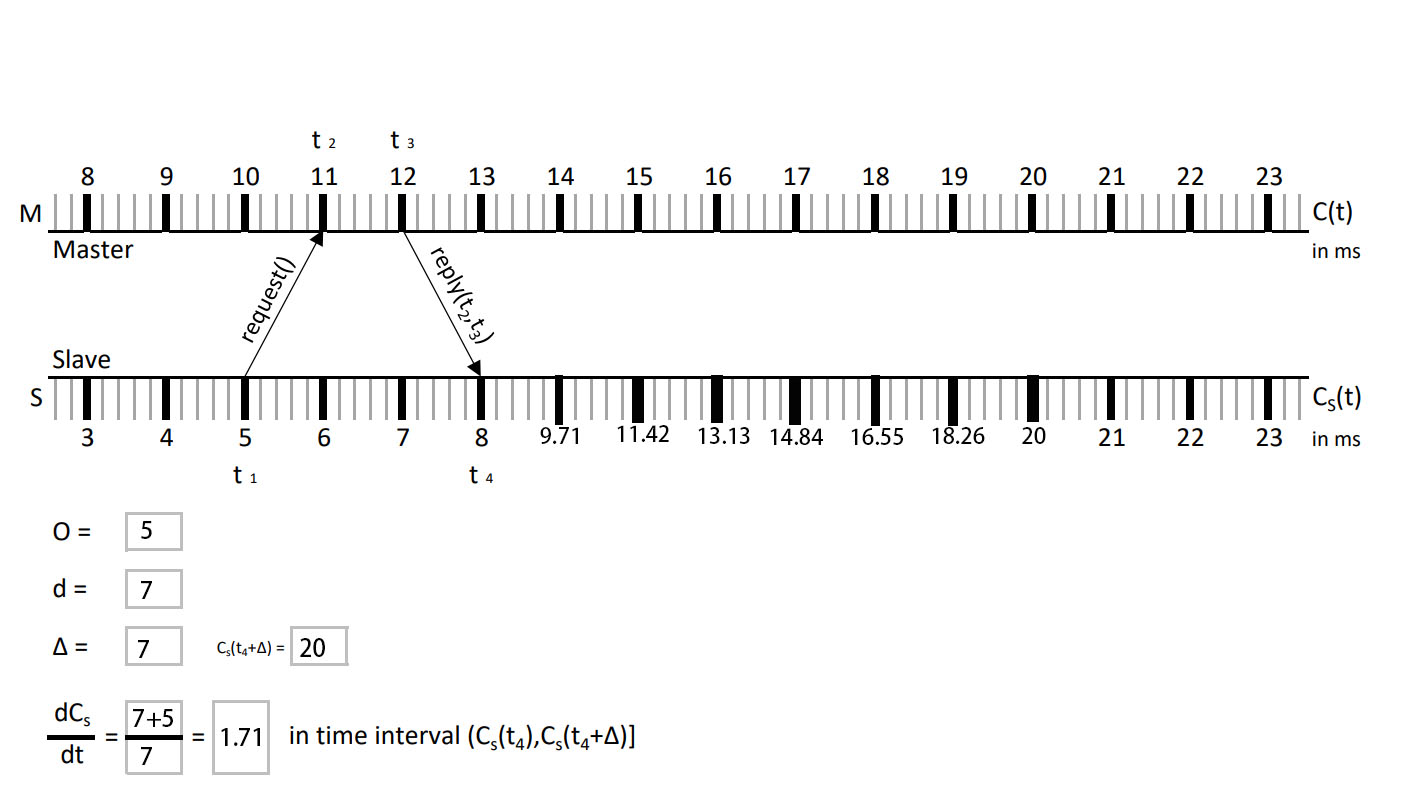
\includegraphics[scale=0.5]{f1.jpg}
\subsection*{b)}
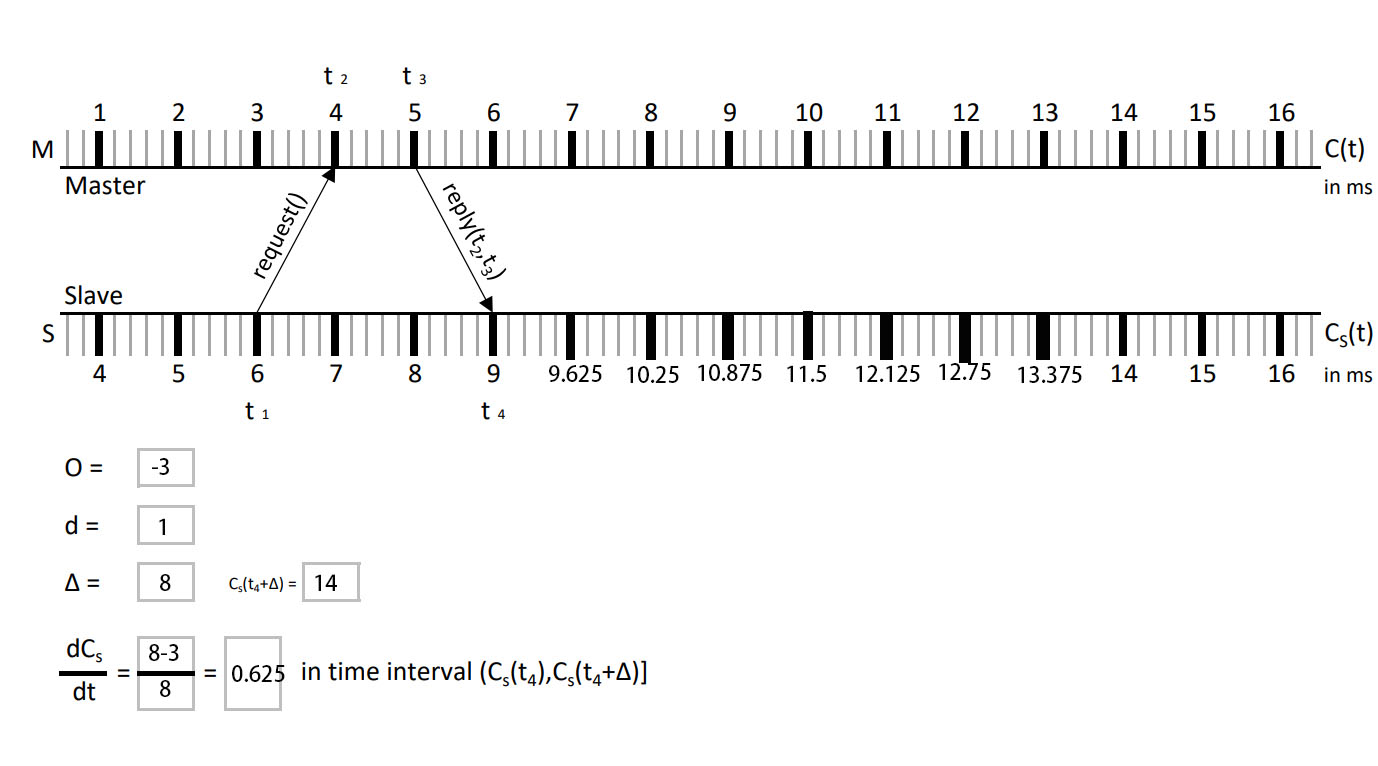
\includegraphics[scale=0.5]{f2.jpg}
\subsection*{c)}
i.send two request and get two reply. Then calculte by this two time.
\[\frac{t_7-t_3}{t_{15}-t_{10}}=0.8\]
ii.
\section{Logical Clocks}
\subsection*{a)}
i. \[e_1^1,e_3^1,e_1^2,e_1^3,e_2^1,e_3^2,e_2^2,e_3^3,e_2^3,e_1^4,e_2^4,e_3^4\]
ii.
\[e_1^1=(1,0,0),e_3^1=(0,0,1),e_1^2=(2,0,1),e_1^3=(3,0,1),e_3^2=(0,0,2),e_3^3=(0,0,3),\]
\[e_2^1=(3,1,1),e_2^2=(3,2,1),e_2^3=(3,3,3),e_2^4=(3,4,3),e_1^4=(4,0,1),e_3^4=(3,4,4)\]
iii.\\
$e_1^4$. By the vector Clocks. $e_3^4=(3,4,4)$. Thats  mean all the events from P2 and P3 is related. Only one event form P1 is not related. $e_1^1,e_1^2,e_1^3$ is contributed to $e_3^4$ by $e_1^3->e_2^1$. So only $e_1^4$ is not related.
\subsection*{b)}
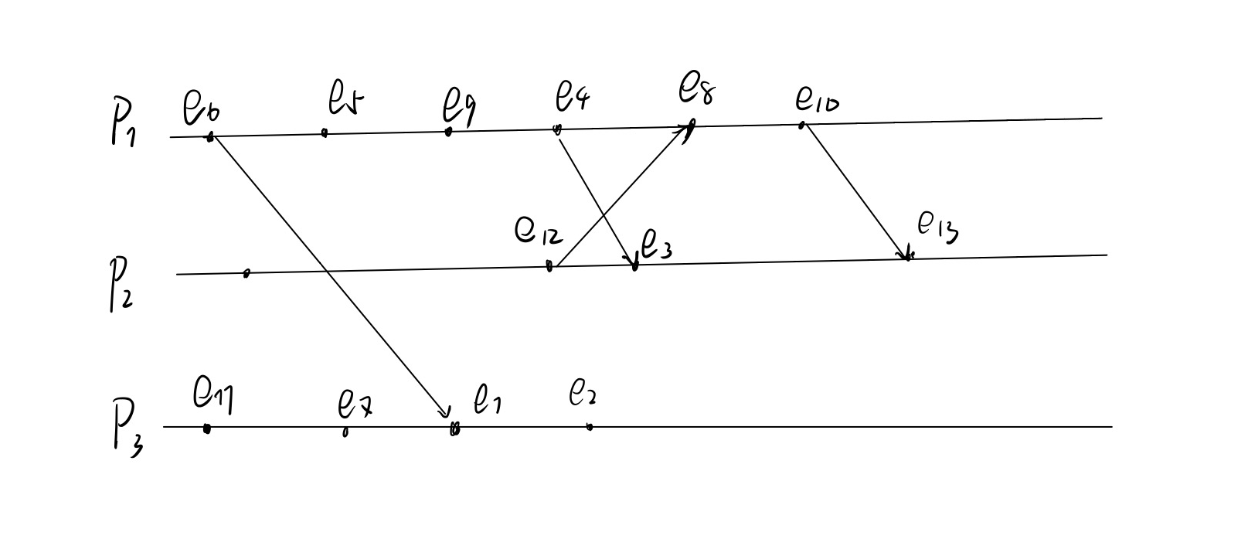
\includegraphics[scale=0.5]{A2b.png}
\section{Global State}
\subsection*{a)}
\[(e^1_1||e_2^1),(e_2^2||e_1^2),(e_1^1||e_2^2),(e_1^2||e_2^1),(e_1^1||e_2^3),(e_1^1,e_2^4),(e_1^2||e_2^3),(e_1^2||e_2^4),(e_2^3||e_1^4)\]
\subsection*{b)}
i.Linearization. All the event is follow the rule happend-before.
\\ii. No Linearization. $e_2^4->e_1^5$ is not follw thw rule happend-before.
\subsection*{c)}
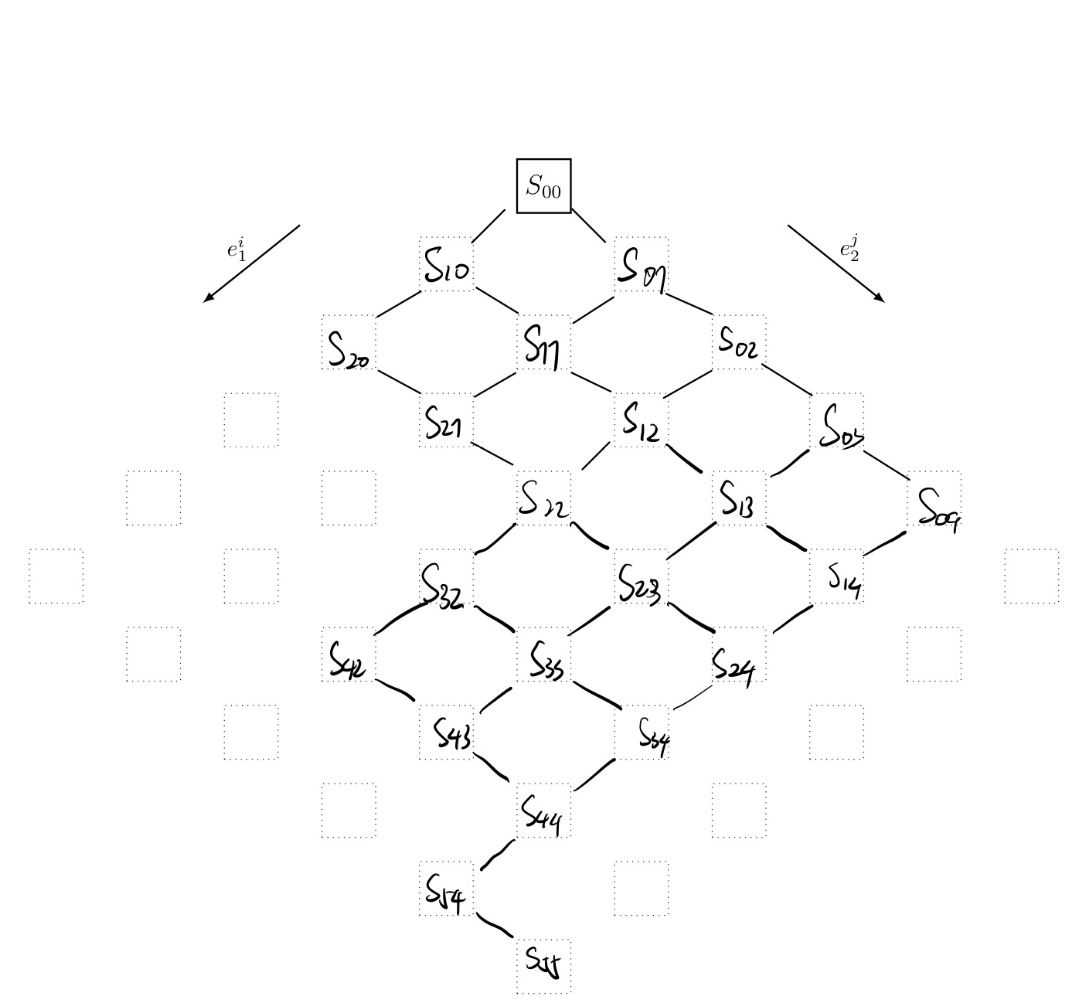
\includegraphics[scale=0.5]{A3C.png}
\section{Snap Algorithm}
\subsection*{a}
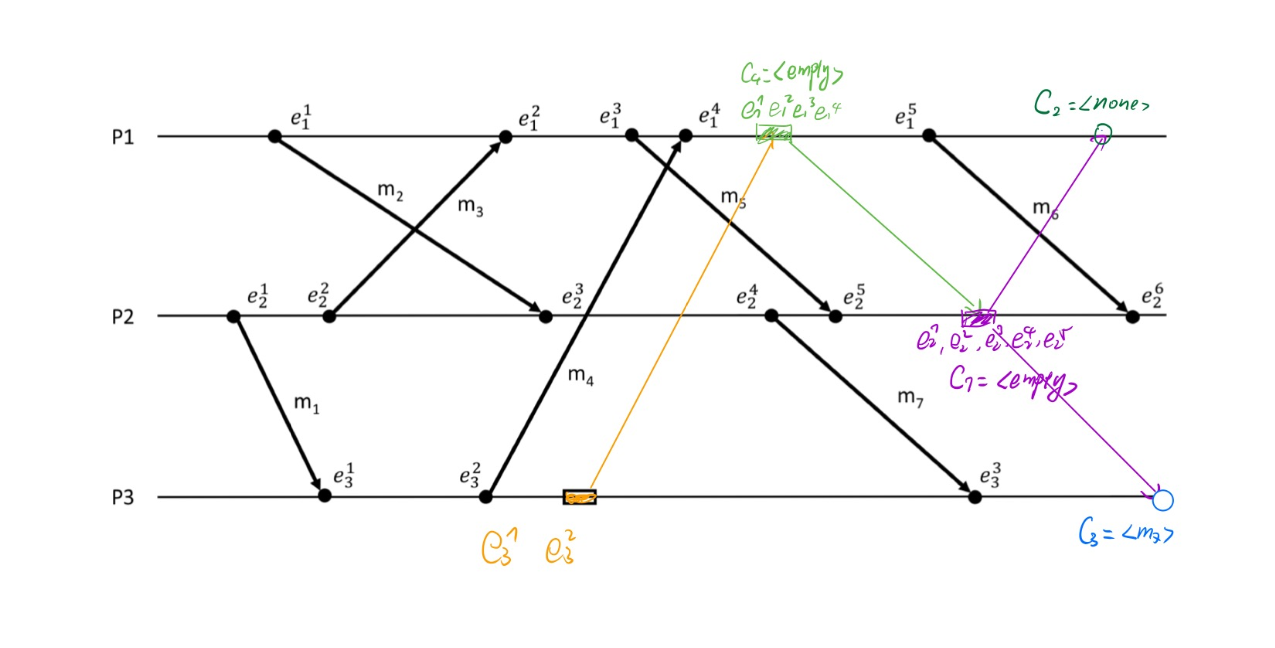
\includegraphics[scale=0.6]{A4.png}
\end{document}
